\chapter{Réalisation du projet}

Ce chapitre est dédié à la concrétisation visuelle et technique de l'application.

\section{Architecture des Microservices et Dépôts (Repositories)}
Conformément aux standards de l'industrie pour les applications Cloud-Native hautement scalables, le code source du projet n'a pas été construit comme un bloc monolithique. Il a été découpé en \textbf{quatre dépôts (repositories) distincts}, représentant chacun un microservice avec une responsabilité métier (Domain-Driven Design) unique :

\subsection{1. Le Frontend : \texttt{enterprise-portal}}
\begin{itemize}
    \item \textbf{Technologie :} React.js, Redux Toolkit, Tailwind CSS.
    \item \textbf{Rôle :} C'est la "vitrine" et l'interface utilisateur (UI) globale. Ce portail unique gère dynamiquement l'affichage selon le rôle de l'utilisateur connecté. Un visiteur B2C verra le catalogue de location de voitures, tandis qu'un directeur (Admin) verra automatiquement apparaître les tableaux de bord de gestion financière. Ce portail communique avec les trois autres microservices backend via des requêtes HTTP (Axios).
\end{itemize}

\subsection{2. Le Backend B2C : \texttt{service-location}}
\begin{itemize}
    \item \textbf{Technologie :} Node.js, Express, MongoDB, Redis.
    \item \textbf{Rôle :} C'est le cœur du métier de Prestige Maroc. Ce microservice gère le catalogue des véhicules, les recherches avec filtres complexes, le tunnel de réservation et la gestion des conflits (Race Conditions) via le verrouillage optimiste. C'est également ce service qui écoute les webhooks de Stripe pour valider les paiements de location.
\end{itemize}

\subsection{3. Le Backend Clients : \texttt{service-crm} (Customer Relationship Management)}
\begin{itemize}
    \item \textbf{Technologie :} Node.js, Express, MongoDB, Nodemailer.
    \item \textbf{Rôle :} Ce service est dédié à 100\% à la gestion des utilisateurs. Il s'occupe de l'inscription, du hachage des mots de passe (Bcrypt), de la génération des Tokens JWT pour la sécurité, et de l'envoi d'emails (récupération de mot de passe, confirmation de compte). En isolant la gestion des utilisateurs, on garantit que même si le service de location tombe en panne, les clients peuvent toujours se connecter à leur profil.
\end{itemize}

\subsection{4. Le Backend Gestion : \texttt{service-erp} (Enterprise Resource Planning)}
\begin{itemize}
    \item \textbf{Technologie :} Node.js, Express, Puppeteer (génération PDF).
    \item \textbf{Rôle :} C'est l'outil back-office réservé à la direction de Prestige Maroc. Ce microservice lourd génère les factures PDF, calcule le chiffre d'affaires, gère la comptabilité et produit les statistiques D3.js affichées dans l' \texttt{enterprise-portal}. Le traitement des factures étant très gourmand en ressources processeur (CPU), son isolation dans le dépôt \texttt{service-erp} permet de ne pas ralentir les clients qui essaient de réserver des voitures sur le \texttt{service-location}.
\end{itemize}

\section{Explication des Principales Pages et Fonctionnalités}

\subsection{Page d'Accueil et Liste des Biens (Véhicules)}
\begin{figure}[H]
    \centering
    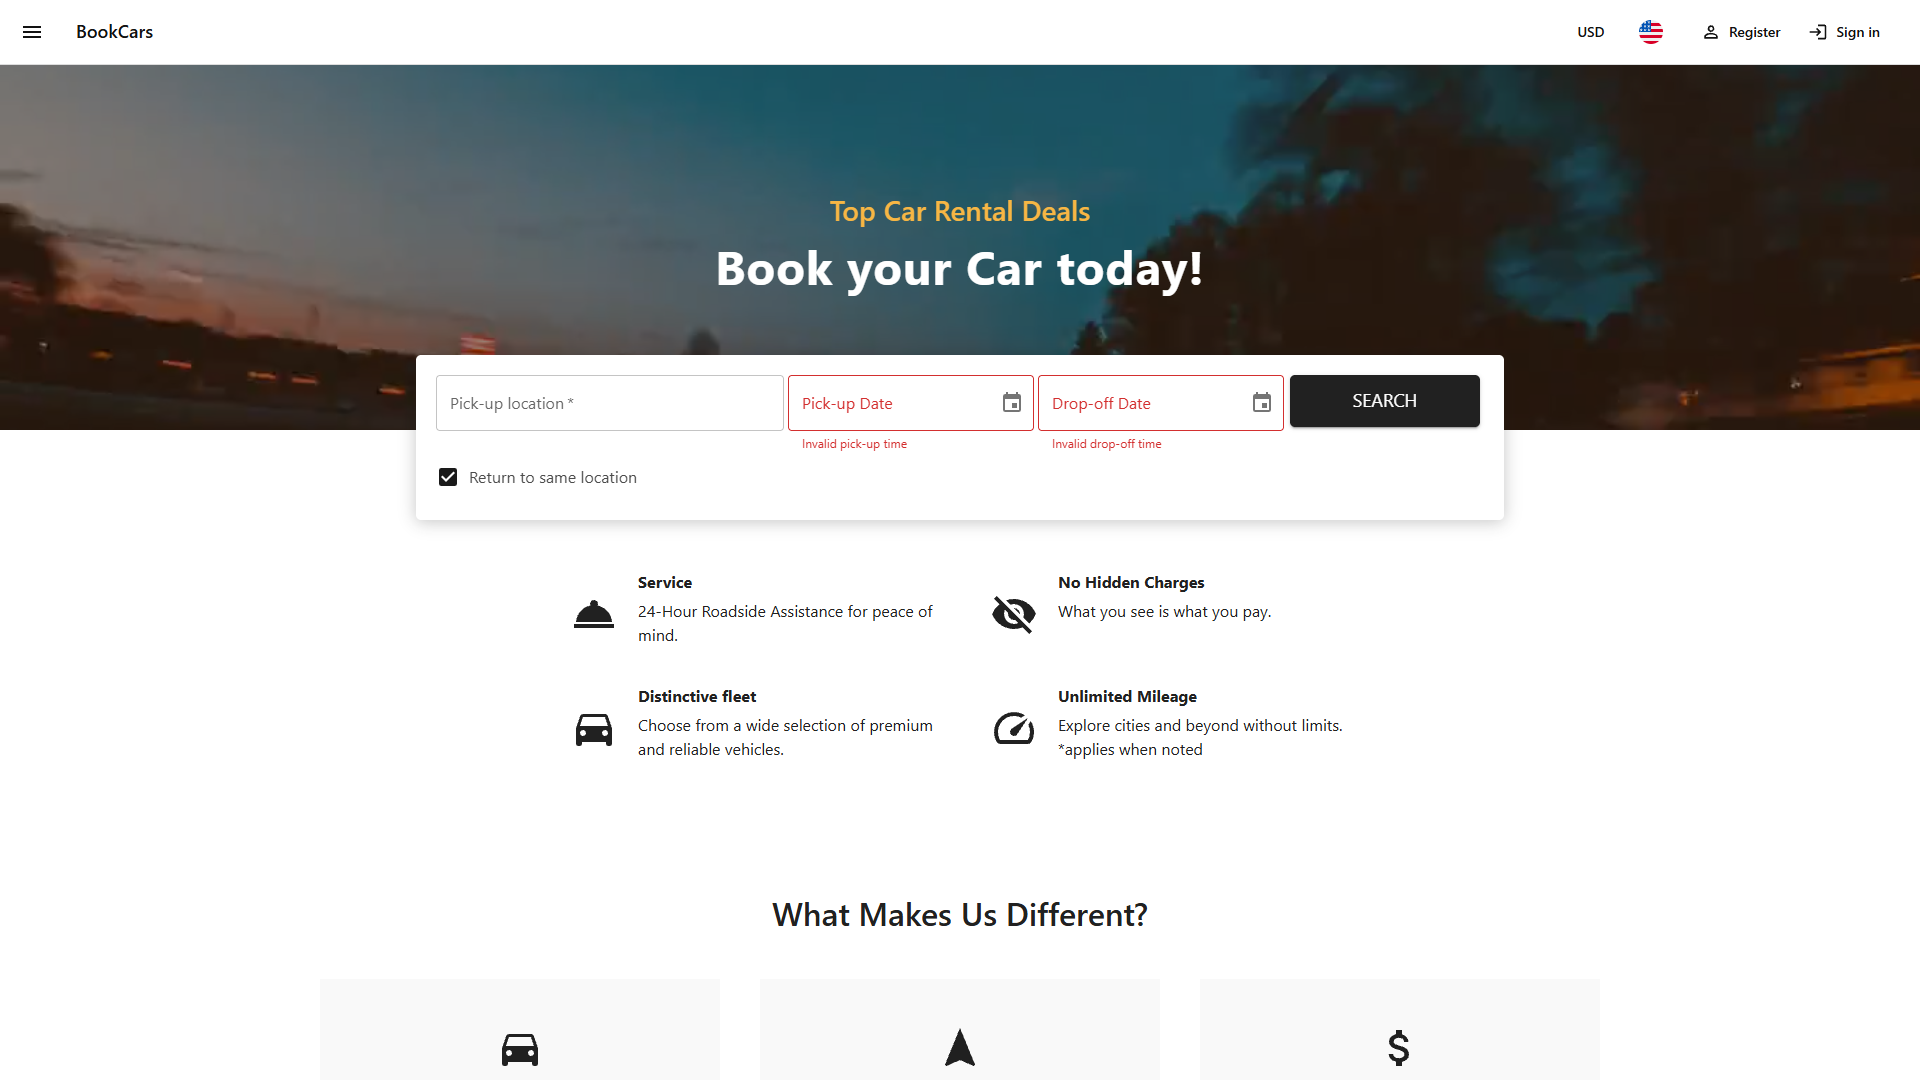
\includegraphics[width=0.9\textwidth]{images/capture_accueil.png}
    \caption{Page d'accueil du portail B2C (Prestige Maroc)}
\end{figure}
\textbf{Explication :} La page d'accueil B2C arbore un design émotionnel. Les véhicules sont affichés via des "Cards" Bootstrap/AntD. L'utilisateur peut filtrer en temps réel par marque ou par prix. \\
\textbf{Mécanique Backend :} Pour afficher le catalogue instantanément (en moins de 50ms), j'ai implémenté un système de **Mise en Cache avec Redis**. Au lieu de solliciter la base de données MongoDB à chaque visite, les données des véhicules sont stockées dans la RAM du serveur.

\subsection{Page de Détail d'un Bien}

\textbf{Explication :} Cette page présente la galerie photo du véhicule, ses caractéristiques (boîte automatique, carburant) et un calendrier interactif pour choisir les dates.
\textbf{Mécanique Backend :} Afin d'optimiser le référencement naturel (SEO) sur Google, cette page utilise le **Server-Side Rendering (SSR)**. Le code HTML est généré côté serveur avant d'être envoyé au navigateur.

\subsection{Page de Connexion / Inscription (Sécurité JWT)}

\textbf{Explication :} Interface épurée permettant au client de s'identifier. \\
\textbf{Mécanique Backend :} Lors de l'inscription, le mot de passe est haché avec l'algorithme \textbf{Bcrypt} (Salt Round 10) avant d'être sauvegardé. Lors de la connexion, le serveur génère un \textbf{JSON Web Token (JWT)} signé cryptographiquement. Ce token est stocké dans les cookies sécurisés du navigateur et permet de maintenir la session active sans surcharger le serveur.

\subsection{Formulaire de Réservation et Paiement (Webhooks)}

\textbf{Explication :} Le client saisit ses informations bancaires pour bloquer le véhicule. \\
\textbf{Mécanique Backend :} C'est la fonctionnalité la plus critique. Pour éviter qu'une même voiture soit louée par deux personnes à la même milliseconde, j'ai implémenté un algorithme de \textbf{Verrouillage Optimiste (Optimistic Locking)}. De plus, le paiement est géré de manière asynchrone : au lieu d'attendre la réponse de la banque, Node.js écoute un \textbf{Webhook Stripe} qui le notifie en arrière-plan lorsque les fonds sont réellement transférés, sécurisant ainsi l'entreprise contre la fraude.

\subsection{Tableau de bord Administrateur (Dashboard)}

\textbf{Explication :} Destiné au directeur de Prestige Maroc. Affiche les statistiques (Chiffre d'affaires, Taux de rotation de la flotte) via des graphiques D3.js. \\
\textbf{Mécanique Backend :} L'accès à cette page est protégé par un \textbf{Contrôle d'Accès Basé sur les Rôles (RBAC)}. Le middleware Node.js intercepte chaque requête, décode le token JWT, et vérifie si l'utilisateur possède le statut \texttt{role: 'ADMIN'}. Dans le cas contraire, une erreur "403 Forbidden" est retournée.

\subsection{Gestion des Annonces et Facturation (ERP)}

\textbf{Explication :} Interface de type "Datatable" permettant de créer (CRUD) des véhicules et d'éditer des factures PDF pour les clients B2B. \\
\textbf{Mécanique Backend :} La génération d'un PDF de plusieurs Mo est déléguée à des \textbf{Worker Threads} (processus en arrière-plan) pour ne pas bloquer le serveur principal (Event Loop) et garantir que le reste du site reste fluide pour les autres clients.

\subsection{Page Contact et Support Client}

\textbf{Explication :} Un formulaire simple permettant aux visiteurs de poser des questions ou de signaler un problème technique. \\
\textbf{Mécanique Backend :} Lors de la soumission du formulaire, Node.js utilise la librairie \textbf{Nodemailer} couplée à un serveur SMTP (ex: SendGrid) pour acheminer l'email directement dans la boîte de réception de l'agence Prestige Maroc, avec une protection anti-spam (reCAPTCHA) implémentée en amont.

\section{DevOps : Intégration et Déploiement Continus (CI/CD)}
L'un des défis majeurs d'un projet moderne est la mise en production sans interrompre le service. J'ai implémenté un pipeline \textbf{CI/CD} en utilisant \textbf{GitHub Actions}.
\begin{itemize}
    \item \textbf{Intégration Continue (CI) :} À chaque fois que je pousse (push) du nouveau code sur GitHub, un serveur automatisé lance la suite de tests Jest. Si un test échoue, le déploiement est annulé.
    \item \textbf{Déploiement Continu (CD) :} Si les tests réussissent, GitHub Actions "build" les conteneurs Docker (un pour React, un pour Node.js) et les déploie automatiquement sur notre Serveur Privé Virtuel (VPS). Cela permet de livrer des mises à jour en quelques minutes sans effort manuel.
\end{itemize}
